
\documentclass[12pt]{article}
\usepackage{geometry} % see geometry.pdf on how to lay out the page. There's lots.
\geometry{a4paper} % or letter or a5paper or ... etc
% \geometry{landscape} % rotated page geometry
\usepackage{color}
\usepackage{apacite}
\usepackage{graphicx}
\usepackage{float}

% See the ``Article customise'' template for some common customisations

%%% BEGIN DOCUMENT
\begin{document}

%Title page
\noindent
Freie Universitat Berlin\\
FB Informatics / Mathematics\\
Cognitive Systems Seminar\\
Winter Term 2018/19\\
Instructor: Ana-Maria Olteteanu
\vspace{5cm}
\begin{center}
{\LARGE \textbf{Essay about a computational model of visual analogies in design}}
\end{center}
\vspace{8cm}

\noindent
Cedric Laier \\
Warschauer Str. 15, 10243 Berlin \\
cedric.laier@fu-berlin.de\\
Informatik, Master (Freie Universität Berlin) \\
5153575 \\
\clearpage


\section{Introduction}

\noindent This essay focuses on a study conducted on the research of problem solving by using visual analogies. The particular paper I want to talk about here is: "A computational model of visual analogies in design" \cite{davies2009computational}. The research goal of this paper was to examine the role of visuospatial knowledge in enabling
the transfer of the problem-solving procedure from the source to the target. \\
\indent An \textit{analogy} itself is the process of finding and using correspondences between concepts. The term \textit{visuospatial} refers to the ability of represent, analyse, and mentally manipulate objects; \textit{transfer} is the application of knowledge from the source analogue to the target analogue. Research has shown that visual analogies, which are part of visual reasoning with visual knowledge, are an important role when it comes to design. Goldman and Casakin have even described visual analogies, on a basis of case studies performed on architectural design, as a core design strategy in architectural design \cite{casakin1999expertise}. That's why Davies, Goel and Nersesian hypthothise in their publication that visuospatial representation of intermediate knowledge states, organized in chronical order can enable transfer of problem solving-procedures. The idea is that by looking a visual representation (let's say drawn with a pen on a piece of paper) of a solution for a given problem, humans are able to transfer the just yet learned knowledge and use an it to draw correspondences between the solution and a new upcoming problem. In the next paragraph you find an example, where we have a written description and a sketch solution for the problem. So we as humans gained new knowledge for this particular problem and might be able to use this knowledge for a similar problem. The goal now is to find out is if visual perception of the spatial relationships of objects from the solution can contribute to solve a 
problem by using an analogy. \\
\indent An example for using this kind of visual analogy for problem solving is by taking the classical fortress and tumour problem \cite{duncker1926qualitative} and sketching it as done by Davies and Goel \cite{davies2001visual}. The participants got a task to read the story about a problem solving situation: A general with a large army wants to overthrow a dictator who lives in a fortress. All roads to the fortress are armed with mines that will go off if many people are on them at the same time. Figure \ref{fig:fortress} shows the initial situation. To solve this problem he breaks up his army into small groups and has them take different roads as seen in Figure \ref{fig:fortress_solution}. The groups arrive at the same time and take the fortress.  
\begin{figure}[H]
    \centering
    \begin{minipage}[b]{0.4\textwidth}
    	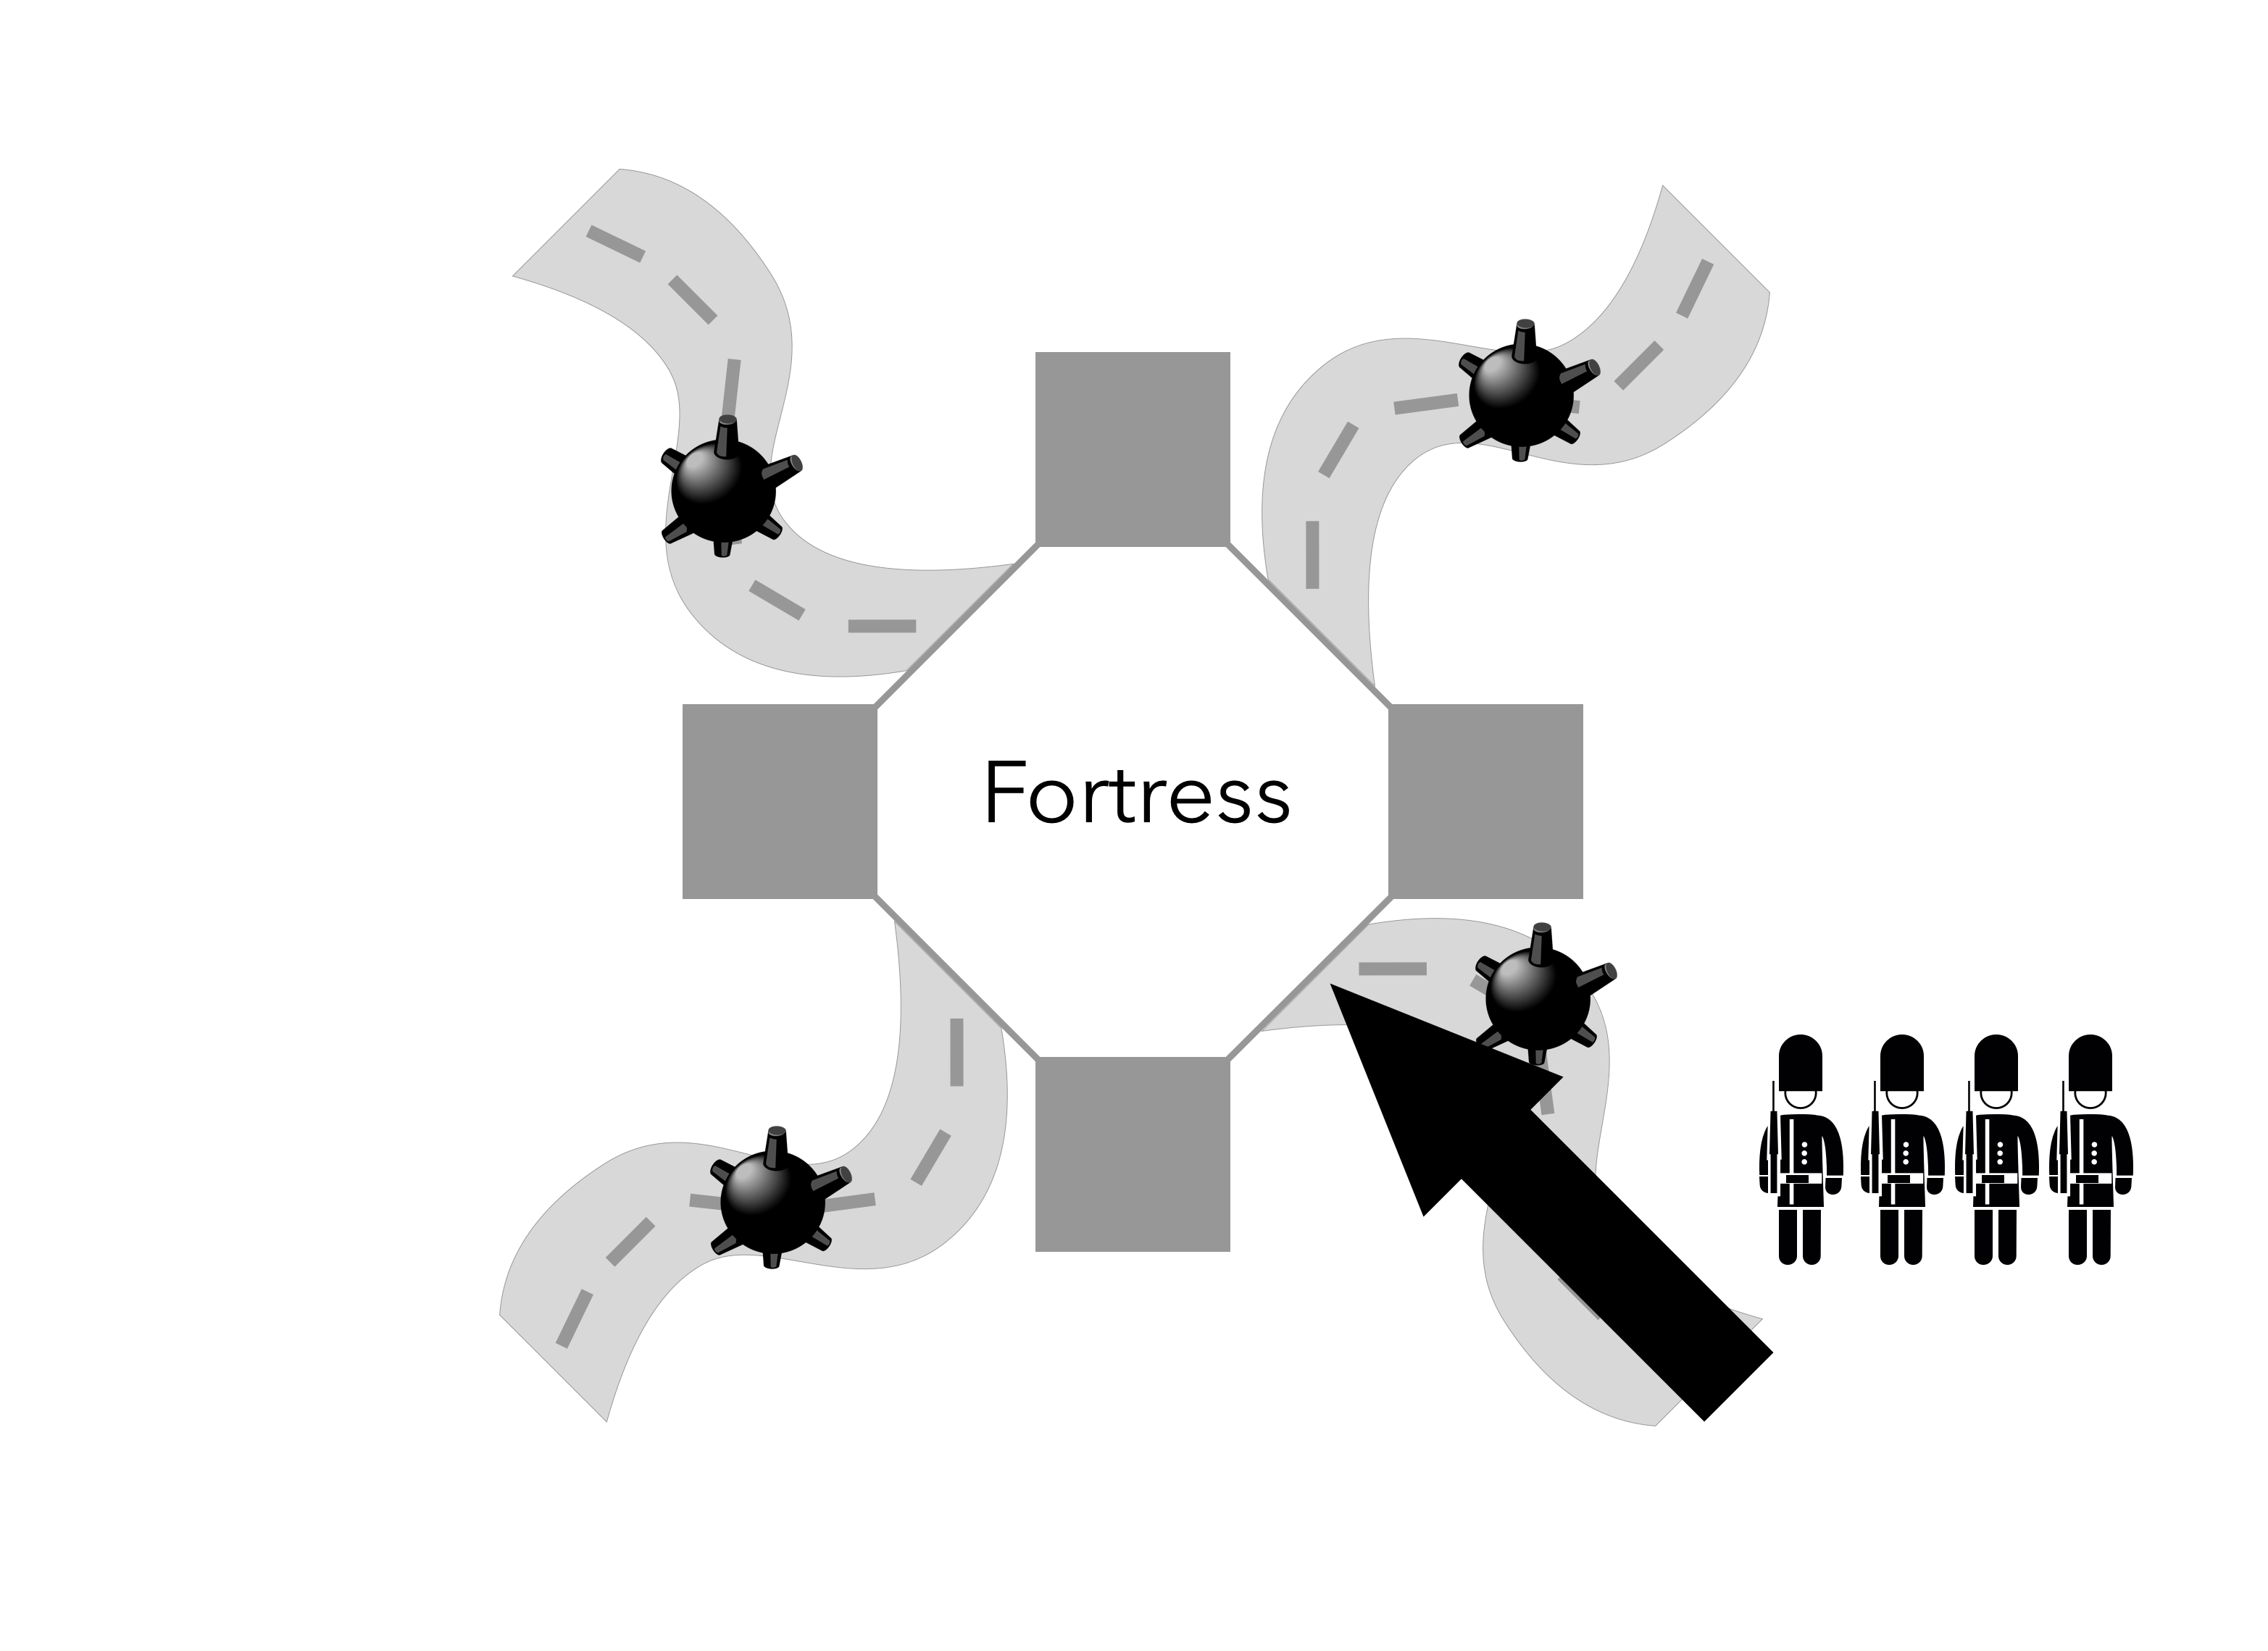
\includegraphics[scale=0.08]{images/fortress_problem.png}
    	\caption{Initial situation of the fortress problem}
    	\label{fig:fortress}
    \end{minipage}
    \hfill
    \begin{minipage}[b]{0.4\textwidth}
    	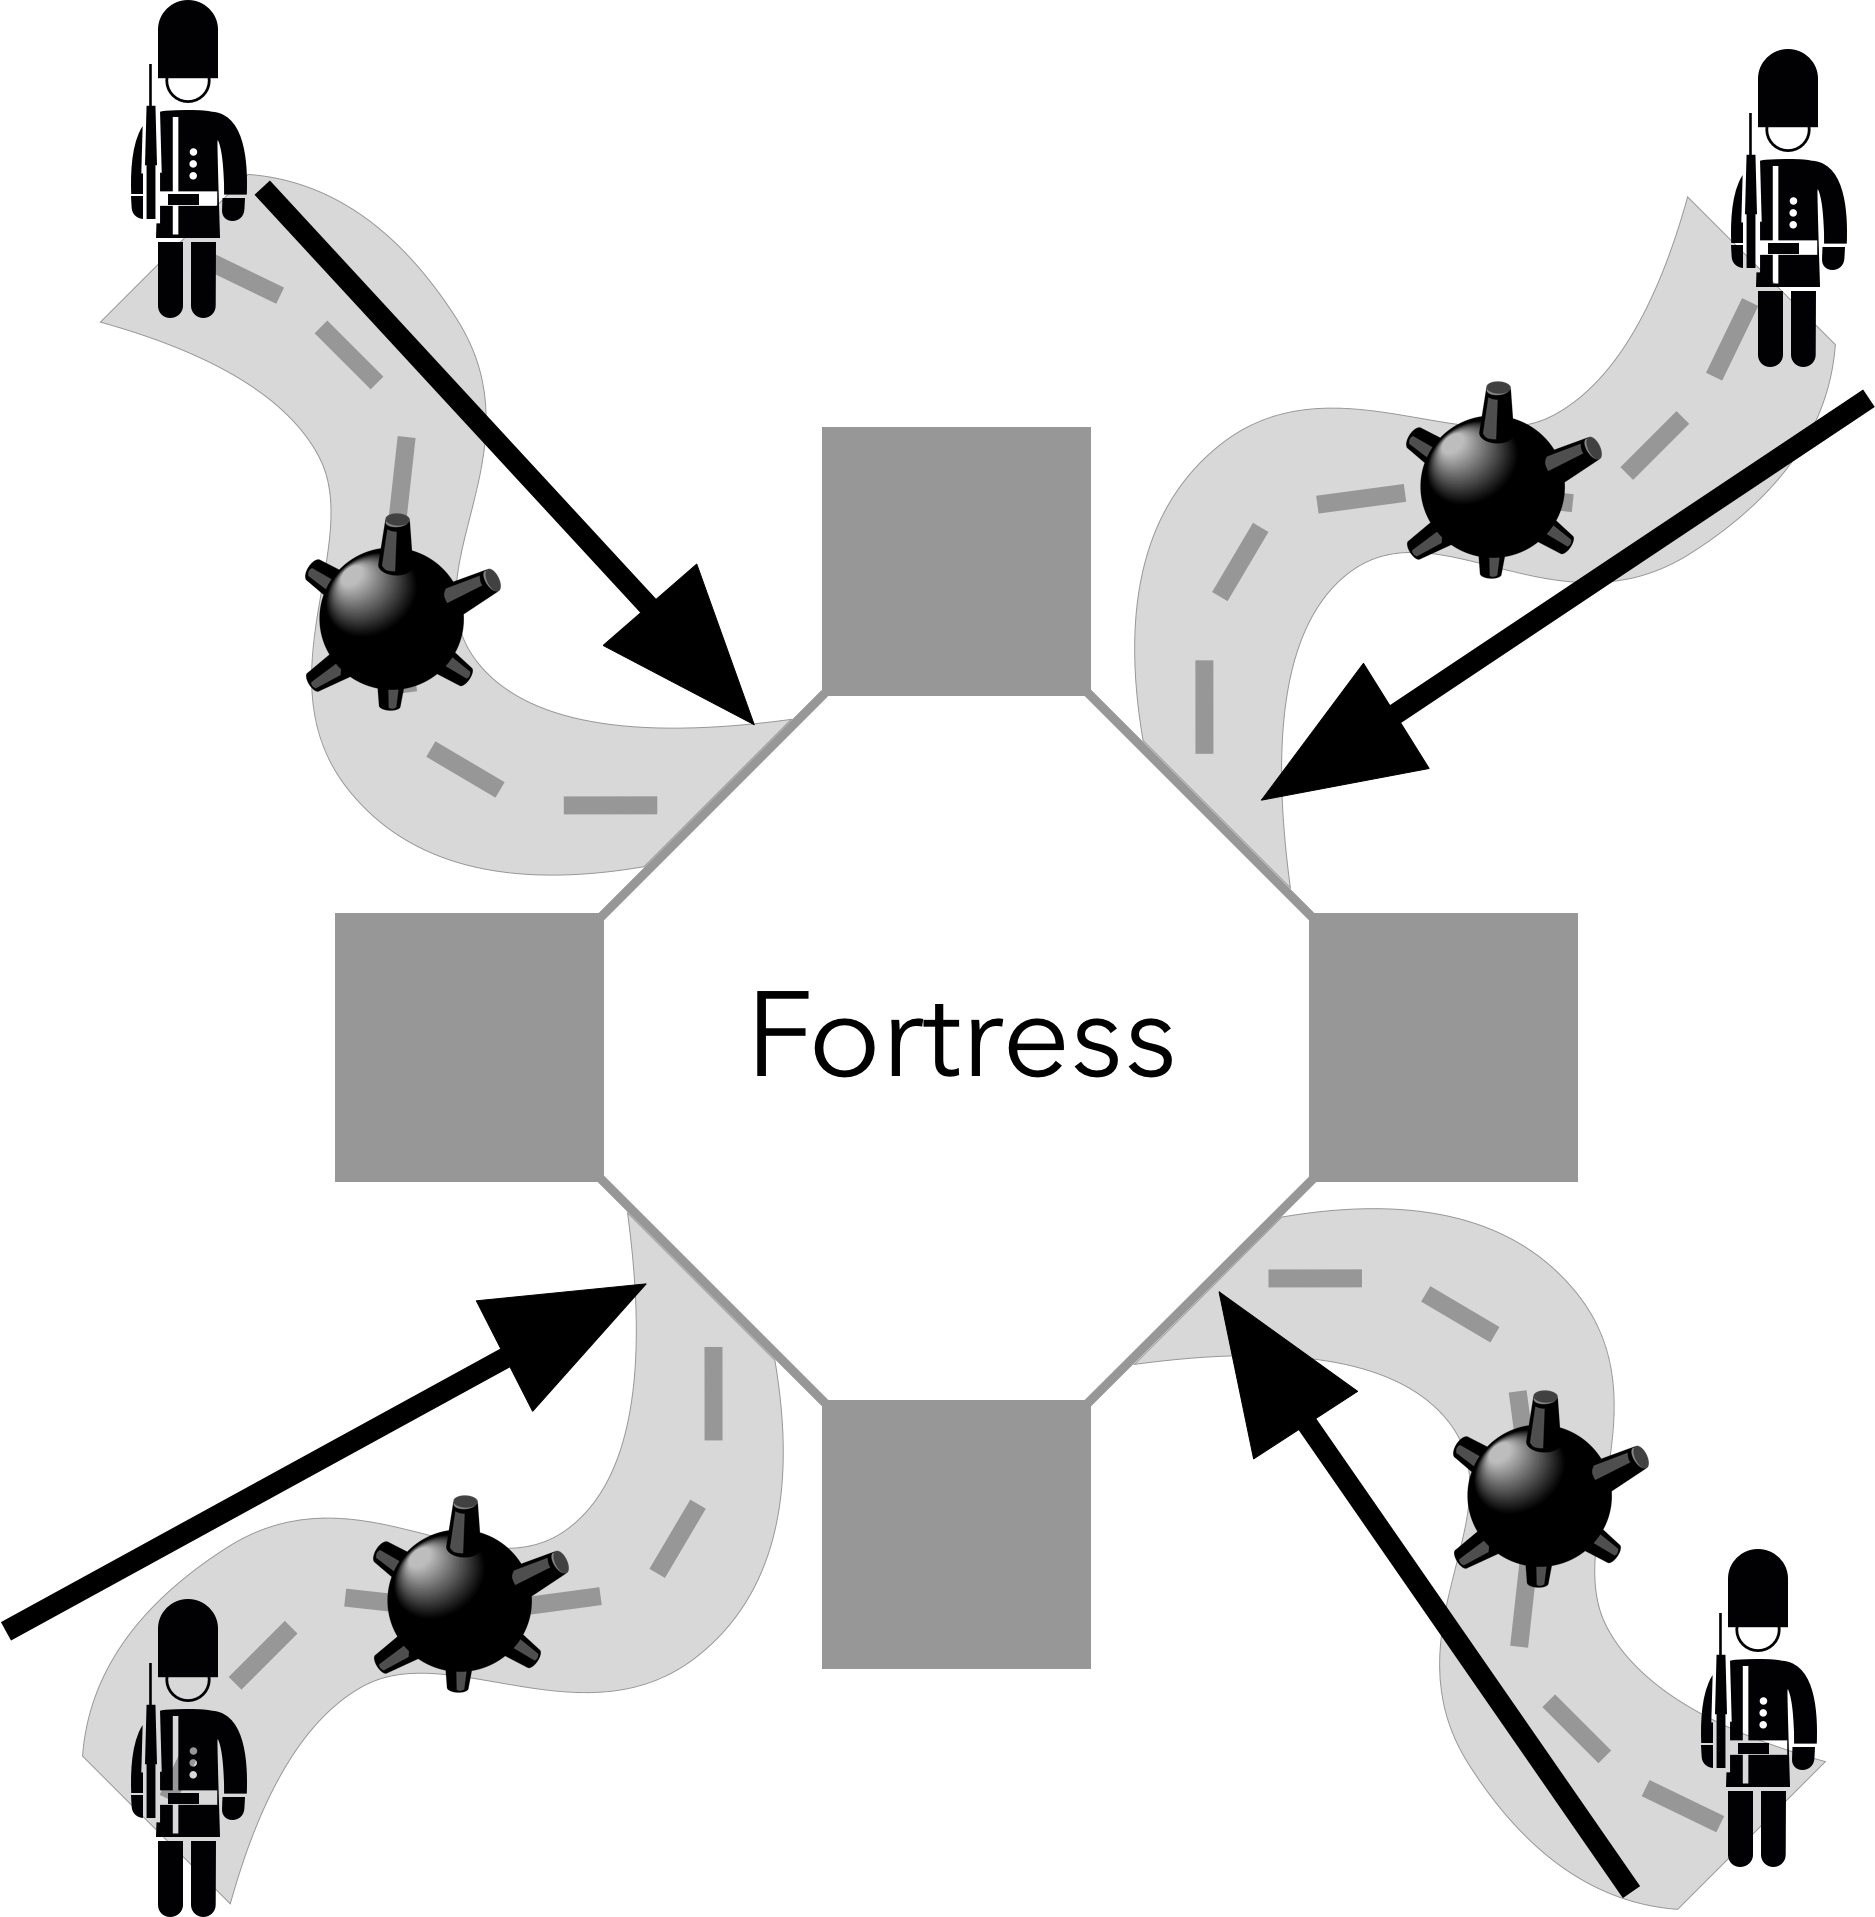
\includegraphics[scale=0.08]{images/fortress_problem_solution.png}
    	\caption{Solution for the fortress problem}
    	\label{fig:fortress_solution}
    \end{minipage}
\end{figure}

Now they get a new different problem as stated as from Gick and Holyoak \cite[307-308]{gick1980analogical}: "Suppose you are a doctor faced with a patient who has a malignant tumour in his stomach. It is impossible to operate on the patient, but unless the tumour is destroyed the patient will die. There is a kind of ray that can be used to destroy the tumour. If  the rays reach the tumour all at once at a sufficiently high intensity, the tumour will be destroyed. Unfortunately, at this intensity the healthy tissue that the rays pass through on the way to the tumour will also be destroyed. At lower intensities the rays are harmless to healthy tissue, but they will not affect the tumour either. What type of procedure might be used to destroy the tumour with the rays, and at the same time avoid destroying the healthy tissue?". Finally, the participants are asked to solve the tumour problem. The expected behaviour is now that the participants are able to find a solution by looking at the sketch and use an analogy they've learned from the fortress problem before. Figure \ref{fig:fortress_solution} illustrates again the initial scenario.

\section{Overview of Research}
Basis of the analysis performed was Craigs \cite{craig2003perceptual} doctorical publication about 34 novice designers from the Georgia Institute of Technologie.


\section{Discussion / Critical Evaluation}
Please discuss the research you reviewed in the above section. For instance,
\begin{itemize}
\item What's good about it?
\item What has been achieved?
\item To what extent does it live up to its aspirations?
\item Take up concerns / comments mentioned during corresponding seminar sessions.
\item How is this research related to other aspects / topics treated in the scope of the seminar?
\end{itemize}

\noindent
\textcolor{red}{Regular term papers should be around  ca.\ 4500 words. \\[2mm] Follow the APA Publication Manual for citation format, both within the text and in the reference list (examples below).}

\nocite{allen:99,allport:94,cranach:80}

\bibliographystyle{apacite}

\bibliography{bib}

\end{document}